\documentclass[a4paper,10pt,twoside]{article}
\usepackage[utf8x]{inputenc}
\usepackage[english]{babel} 
\usepackage[usenames,dvipsnames,figures]{xcolor}
\usepackage{lmodern,tikz,makeidx,graphicx,eurosym,amsmath,comment,titlesec,subcaption,textgreek,multirow,hyperref,url,enumerate,chemfig,sectsty,mathrsfs,amssymb,amsthm,multicol,fancyhdr,setspace,indentfirst,multicol,gensymb,textcomp,booktabs,bookmark}
\usepackage[neverdecrease]{paralist}
\usepackage[authoryear]{natbib}
\usepackage[autostyle]{csquotes}  
\usepackage[final]{pdfpages}
\usepackage{mhchem}
\usepackage[top=3cm, bottom=3cm, left=3cm, right=3cm]{geometry}
\usepackage[linesnumbered,ruled]{algorithm2e}

\newtheorem{theorem}{Theorem}

\RequirePackage{amsmath,amssymb,latexsym}
\hypersetup{
    colorlinks=false,       % false: boxed links; true: colored links
    linkcolor=black,          % color of internal links (change box color with linkbordercolor)
    citecolor=black,        % color of links to bibliography
    filecolor=black,      % color of file links
    urlcolor=black           % color of external links
}

\setlength\columnsep{26pt}

\newcommand\norm[1]{\left\lVert#1\right\rVert}

\pagestyle{fancy}
\setlength{\headheight}{25pt} 
\lhead{\textbf{Philip Hartout}}
\rhead{\textbf{Introduction to Machine Learning - Summary}}
\rfoot{}

\newcommand{\HRule}{\rule{\linewidth}{0.5mm}} 
\newcommand{\angstrom}{\mbox{\normalfont\AA}}
\newlength{\drop}
\newtheorem{definition}{Definition}[section]

\title{Introduction to Machine Learning \\ Summary}
\author{Philip Hartout}
\date{\today}   

\begin{document}

\maketitle

\tableofcontents

\section{Linear Regression}
Objective, approximate:
\begin{align*}
    f(x) &= w_1x_1+\ldots+w_dx_d+w_0\\
        &= \sum_{i=1}^{d}w_ix_i+w_0\\
        &= \mathbf{w}^{T}\mathbf{x}+w_0
\end{align*}
$\forall \mathbf{x}, \mathbf{w}\in\mathbb{R}^{d}$. This expression can be further compressed to the homogeneous representation where $\forall \mathbf{\tilde{x}}, \mathbf{\tilde{w}}\in\mathbb{R}^{d+1}$, i.e. $\tilde{x}_{d+1}=1$. We have w.l.o.g.:
\begin{align*}
f(x) = \mathbf{w}^{T}\mathbf{x}
\end{align*}
Quantify errors using residuals:
\begin{align*}
    r_i &= y_i-f(x_i)\\
        &= y_i-\mathbf{w}^{T}\mathbf{x_i}
\end{align*}
We can use squared residuals and sum over all residuals to get the cost:
\begin{align}
    \label{objective_lse}
    \hat{R}(w) &= \sum_{i=1}^{n}r_i^2\\
               &= \sum_{i=1}^{n}(y_i-\mathbf{w}^{T}\mathbf{x_i})^2
\end{align}
Optimization objective to find optimal weight vector $\mathbf{w}$ with least squares is the following:
\begin{equation*}
    \mathbf{w} = \arg\min_{\mathbf{w}}\displaystyle\sum_{i=1}^{n}\left(y_i-w^{T}x_i\right)^2
\end{equation*}

\subsection{Closed form solution}
This can be solved in closed form:
\begin{equation*}
    \mathbf{\hat{w}} = (\mathbf{X}^{T}\mathbf{X})^{-1}\mathbf{X}^{T}\mathbf{y}
\end{equation*}

where:
\begin{equation*}
    X = 
    \begin{bmatrix}
        X_{1,1} & \ldots & X_{1,d}\\
        \vdots & \ddots & \vdots\\
        X_{n,1} & \ldots & X_{n,d}\\
    \end{bmatrix}        
    \text{ and }
    y = 
    \begin{bmatrix}
        y_{1} \\
        \vdots \\
        y_{n}
    \end{bmatrix}
\end{equation*}

\subsection{Optimization}
\subsubsection{Requirements}
Requires a convex objective function.
\begin{definition}[Convexity]
    A function is convex iff $\forall \mathbf{x},\mathbf{x}', \lambda\in[0,1] \text{ it holds that } f(\lambda x+(1-\lambda)x')\leq \lambda f(x)+(1-\lambda)f(x')$
\end{definition}
Note that the least squares objective function defined in \ref{objective_lse} is convex. 
\subsubsection{Gradient descent}
We start with an arbitrary $w_0\in\mathbb{R}^d$, then for $t=0,1,2,\ldots$ we perform the following operation:
\begin{equation*}
    w_{t+1} = w_t -\eta_t\nabla\hat{R}(w_t)
\end{equation*}
where $\eta_t$ is the learning rate.\\
Under mild assumptions, if the step size is sufficiently small, the gradient descent procedure converges to a stationary point, where the gradient is zero. For convex objectives, it therefore finds the optimal solution. In the case of the squared loss and a constant step size (e.g. 0.5), the algorithm converges at linear rate. If you look at the difference in empirical value at iteration $t$ and compare that with the optimal value, then the gap is going to shrink at linear rate. If we look for a solution within a margin $\epsilon$, it is found in $\mathcal{O}(\ln(\frac{1}{\epsilon}))$ iterations.  The fact that the objective function congerges at linear rate can be formally described 
as follows:

\begin{equation*}
    \exists t_0 \forall t\geq t_0, \exists \alpha<1 \text{ s.t. } (\hat{R}(w_{t+1})-\hat{R}(\hat{w}))\leq\alpha(\hat{R}(w_{t})-\hat{R}(\hat{w}))
\end{equation*}

where $\hat{w}$ is the optimal value for the hyperparameters.\\
For computing the gradient, we recall that:
\begin{equation*}
    \nabla\hat{R}(\hat{w}) = 
    \begin{bmatrix}
        \frac{\partial}{\partial w_1}\hat{R}(w) & \ldots & \frac{\partial}{\partial w_d}\hat{R}(w)
    \end{bmatrix}
\end{equation*}
In one dimension, we have that:
\begin{align*}
    \nabla\hat{R}(w) &= \frac{d}{dw}\hat{R}(w) = \frac{d}{dw}\sum_{i=1}^{n}(y_i-w\cdot x_i)^2\\
    &= \sum_{i=1}^{n}\frac{d}{dw}(y_i-w\cdot x_i)^2\\
    &=2(y_i-w\cdot x_i)\cdot(-x_i)\\
    &=\sum_{i=1}^{n}2(y_i-w\cdot x_i)\cdot(-x_i)\\
    &=-2\sum_{i=1}^{n}r_i x_i.\\
\end{align*}
In $d$-dimension, we have that:
\begin{equation*}
    \nabla\hat{R}(w)=-2\sum_{i=1}^{n}r_i x_i,
\end{equation*}
where $r_i\in\mathbb{R}$ and $x_i\in\mathbb{R}^d$

\subsubsection{Adaptive step size for gradient descent}

The step size can be updates adaptively, via either:
\begin{enumerate}
    \item \textbf{Line search}:\\
    Suppose at iteration $t$, we have $w_t$, $g_t=\nabla\hat{R}(w_t)$. We then define:
    \begin{equation*}
        y_t^{*} = \arg\min_{y\in[0,\infty)}\hat{R}(w_t)-\eta g_t
    \end{equation*}
    \item \textbf{Bold driver heuristic}:
    \begin{itemize}
        \item If the function decreases, increase the step size.
        \begin{equation*}
            \text{If }\hat{R}(w_{t+1})<\hat{R}(w_{t}): \eta_{t+1}\leftarrow\eta_{t}\cdot c_{acc}
        \end{equation*}
        where $c_{acc}>1$
        \item If the function increases, decrease the step size. 
        \begin{equation*}
            \text{If }\hat{R}(w_{t+1})>\hat{R}(w_{t}): \eta_{t+1}\leftarrow\eta_{t}\cdot c_{dec}
        \end{equation*}
        where $c_{dec}<1$.
    \end{itemize}
\end{enumerate}
\subsubsection{Tradeoff between gradient descent and closed form}
Several reasons:
\begin{itemize}
    \item Computational complexity:
    \begin{equation*}
        \hat{w}=(X^TX)^{-1}(X^Ty)
    \end{equation*}
    $(X^TX)$ can be computed in $\mathcal{O}(nd^2)$, $(X^TX)^{-1}$ can be computed in $\mathcal{O}(d^3)$.\\
    By comparison, for gradient descent calculating $\nabla\hat{R}(w)=\sum_{i=1}^{n}(y_i-w^Tx_i)x_i$ can be computed in $\mathcal{O}(nd)$, where $n=\ln(\frac{1}{\epsilon})$
    \item the problem may not require an optimal solution.
    \item many problems do not admit a closed form solution.
\end{itemize}
\subsection{other loss functions}
Least squares is part of a general case of the following general loss function, which is convex for $p\geq 1$.
\begin{equation}
    l_p(r)=|r|^p
\end{equation}
Least squares is where $p=2$.

\section{Probability (interlude)}
\subsection{Gaussians}

The p.d.f. of a Gaussian distribution is given by:
\begin{equation}
    \frac{1}{\sqrt{2\pi\sigma^2}}\exp\left(-\frac{x-\mu}{2\sigma^2}\right)
\end{equation}
The p.d.f. of a multivariate Gaussian distribution is given by:
\begin{equation}
    \frac{1}{2\pi\sqrt{|\sigma|}}\exp\left(-\frac{1}{2}(x-\mu)^T\sigma^{-1}(x-\mu)\right)
\end{equation}
where:
\begin{equation}
    \sigma = \begin{pmatrix}
        \sigma_{1}^2, \sigma_{12}\\
        \sigma_{21}, \sigma_{2}^2
    \end{pmatrix}
    \text{ and }
    \begin{pmatrix}
        \mu_1\\
        \mu_2
    \end{pmatrix}
\end{equation}
\subsection{Expectations}
Expected value of a random variable can be calculated as follows:
\begin{equation*}
    \mathbb{E}=\begin{cases}
        \sum_{x}xp(x)\qquad\text{if }X\text{ is discrete}\\
        \int xp(x)dx\qquad\text{if }X\text{ is continuous}\\
    \end{cases}
\end{equation*}
Expectations respect linear properties, i.e. let $X, Y$ be random variable and 
$a,b\in\mathbb{R}$, then we have $\mathbb{E}[aX+bY]=a\mathbb{E}[X]+b\mathbb{E}[Y]$.

\section{Generalization and model validation}

\subsection{Fitting nonlinear functions via linear regression}

Using nonlinear features of our data (basis functions), we can fit nonlinear functions via linear regression. Then, the model takes on the form:

\begin{equation}
    f(\mathbf{x}) = \sum_{i=1}^{d}w_i\phi(\mathbf{x})
\end{equation}

where $\mathbf{x}\in\mathbb{R}^d$, $x\mapsto \tilde{x}=\phi(\mathbf{x})\in\mathbb{R}^d$ and $w\in\mathbb{R}^d$. 
\begin{itemize}
    \item 1 dim.: $\phi(\mathbf{x})=\begin{bmatrix}
        1,x, x^2, \ldots, x^k
    \end{bmatrix}$
    \item 2 dim.: $\phi(\mathbf{x})=\begin{bmatrix}
        1,x_1, x_2, x_1^2, x_2^2, \ldots, x_1^k, x_2^k
    \end{bmatrix}$
    \item p dim.: $\phi(\mathbf{x})$ vector of all monomials in $x_1,\ldots, x_p$ of degree up to $k$.
\end{itemize}

\subsection{Achieving generalization}
\subsubsection{Independence and identical distribution}
A fundamental assumption needs to be met: the dataset is generated from an independently and identically distributed from some unknown distribution $P$, i.e:
\begin{equation*}
    (x_i, y_i)\sim P(\mathbf{X},Y).
\end{equation*}

The i.i.d. assumption is invalid when:
\begin{itemize}
    \item we deal with time series data
    \item spatially correlated data
    \item correlated noise
\end{itemize}
If violated, we can still use ML but the interpretation of the results needs to be carefully analyzed. The most important thing is to choose the train/test split to assess the desired generalization properties of the trained model. 

\subsection{Expected error and generalization error}
Once the iid assumption is verified, our goal is then to minimize the expected error (true risk) under $P$, i.e.:
\begin{align*}
    R(\mathbf{w})&=\int P(\mathbf{x},y)(y-\mathbf{w}^T\mathbf{x})^2dxdy\\
    & =\mathbb{E}[(y-\mathbf{w}^T\mathbf{x})^2]
\end{align*}
The true risk can be estimated by the empirical risk on a sample dataset $D$:
\begin{equation*}
    \hat{R}_D(\mathbf{w})=\frac{1}{|D|}\sum_{\mathbf{x}, y\in D}(y-\mathbf{w}^T\mathbf{x})^2
\end{equation*}
The reason behind this approximation is because of the law of large numbers
\begin{definition}[Law of large numbers]
    $\hat{R}_D(\mathbf{w})\rightarrow R_D(\mathbf{w})$ for any fixed $\mathbf{w}$ as $|D|\rightarrow\infty$.
\end{definition}
\begin{equation}
    \label{empirical_risk}
    \mathbf{\hat{w}}_D=\arg\min_{\mathbf{w}}\hat{R}_D(\mathbf{w})
\end{equation}

\begin{equation}
    \label{true_risk}
    \mathbf{w*}=\arg\min_{\mathbf{w}}\hat{R}(\mathbf{w})
\end{equation}

We don't want to minimize the empirical risk given in equation \ref{empirical_risk} but the true risk given in equation \ref{true_risk}, which are similar as the amount points in the dataset increases.

\subsection{Uniform convergence}

For learning via empirical risk minimization, uniform convergence is required, i.e.:
\begin{equation*}
    \sup_{\mathbf{w}}|R(\mathbf{w})-\hat{R}_D(\mathbf{w})|\rightarrow 0 \text{ as }|D|\rightarrow\infty
\end{equation*}

Note that this is not implied by the law of large numbers alone, but depends on model class. It holds for instance for squared loss on data distributions with bouded support. Statistical learning theory is required to define these properties.

\subsection{Evaluation of performance on training data}

In general in holds that:
\begin{equation*}
    \mathbb{E}_D[\hat{R}_D(\hat{\mathbf{w}}_D)]\leq\mathbb{E}_D[R_D(\hat{\mathbf{w}}_D)]
\end{equation*}
\begin{proof}[Proof]
    \begin{align*}
        \mathbb{E}[\hat{R}_D(\hat{\mathbf{w}}_D)] &= \mathbb{E}_D[\min_{\mathbf{w}}\hat{R}_D(\mathbf{w})]\qquad\text{(ERM)}\\
        &\leq \min_{\mathbf{w}}\mathbb{E}_D[\hat{R}_D(\mathbf{w})]\qquad\text{(Jensen's inequality)}\\
        &= \min_{\mathbf{w}}\mathbb{E}_D[\frac{1}{|D|}\sum_{i=1}^{|D|}(y_i-wx_i)^2]\qquad\text{(Definition of $\hat{R}_D(.)$)}\\
        &= \min_{\mathbf{w}}\mathbb{E}_D[\frac{1}{|D|}\sum_{i=1}^{|D|}(y_i-wx_i)^2]\qquad\text{(linear expectations)}\\
        &= \min_{\mathbf{w}}R(\mathbf{w})\leq\mathbb{E}[R(\hat{w}_D)]\\
    \end{align*}
\end{proof}
Thus, we obtain an overly optimistic estimate. A more realistic evaluation would be to use a separate test set from the same distribution $P$. Then:
\begin{itemize}
    \item Optimize $w$ on training set:
    \begin{equation*}
        \mathbf{\hat{w}}_{D_{\text{train}}} = \arg\min_{\mathbb{w}} \hat{R}_{\text{train}}(\mathbb{w})
    \end{equation*}
    \item Evaluate on test set:
    \begin{equation*}
        \hat{R}_{\text{test}}(\mathbf{\hat{w}})=\frac{1}{|D_{\text{test}}|}\sum_{\mathbf{x},y\in D_{\text{test}}}^{}(y-\hat{\mathbf{w}}^T\mathbf{x})^2
    \end{equation*}
    \item Then:
    \begin{equation*}
        \mathbb{E}_{D_{\text{train}}, D_{\text{test}}}[\hat{R}_{D_{\text{test}}}(\hat{\mathbf{w}}_{D_{\text{train}}})]=\mathbb{E}_{D_{\text{train}}}[R(\mathbf{\hat{w}}_{D_{\text{train}}})]
    \end{equation*}
\end{itemize}
\begin{proof}[Proof]
    Let $D_train=D$, $D_test=V$ and $D,V\sim P$. Then:
    \begin{align*}
        \mathbb{E}_{D,V}[\hat{R}_V(\hat{\mathbf{w}}_D)] &= \mathbb{E}_D[\mathbb{E}_V[\hat{R}_V(\hat{\mathbf{w}}_D)]]\qquad\text{independence of $D,V$}\\
        &=\mathbb{E}_D[\mathbb{E}_V[\frac{1}{|V|}\sum_{i=1}^{|V|}(y_i-\hat{\mathbf{w}}_D^Tx_i)^2]]\qquad\text{(Definition of $\hat{R}_D(.)$)}\\
        &=\mathbb{E}_D[\frac{1}{|V|}\sum_{i=1}^{|V|}\mathbb{E}_{x_i, y_i}(y_i-\hat{\mathbf{w}}_D^Tx_i)^2]\qquad\text{since $(x_i,y_i)\bot D$}\\
        &=\mathbb{E}_D[R(\mathbf{\hat{w}}_D)]   
    \end{align*}
\end{proof}
\subsection{Evaluation for model selection}
For each candidate model $m$, we repeat the following procedure for $i=1:k$:
\begin{itemize}
    \item We split the same dataset into training and validation sets:
    \begin{equation*}
        D=D_{\text{train}}^{(i)}\biguplus D_{\text{val}}^{(i)}
    \end{equation*}
    \item We train the model:
    \begin{equation*}
        \hat{\mathbb{w}}_[i,m]=\arg\min_{\mathbf{w}}\hat{R}_{\text{train}}^{(i)}(\mathbf{w})
    \end{equation*}
    \item Then we estimate the error:
    \begin{equation*}
        \hat{R}_{m}^{(i)}=\hat{R}_{\text{val}}^{(i)}(\hat{\mathbf{w}}_i)
    \end{equation*}
\end{itemize}
Finally, select the model:
\begin{equation*}
    \hat{m}=\arg\min_{m}\frac{1}{k}\sum_{i=1}^{k}\hat{R}_{m}^{(i)}
\end{equation*}
\subsection{Splitting the data for model selection}
This splitting can be done randomly through Monte Carlo cross-validation. 
\begin{itemize}
    \item Pick training set of given size uniformly at random
    \item Validate on remaining points
    \item Estimate prediction error by averaging the validation error over multiple random trials.
\end{itemize}
It can also be achieved through $k$-fold cross-validation, which is the default choice.
\begin{itemize}
    \item Partition the data into $k$ folds
    \item Train on $k-1$ folds, evaluating on remaining fold.
    \item Estimate prediction error by averaging the validation error obtained while varying the validation fold.
\end{itemize}
Note that the cross-validation error is almost unbiased for large enough $k$. The following should be considered to pick $k$:
\begin{itemize}
    \item Too small: 
    \begin{itemize}
        \item Risk of overfitting on test set
        \item Using too little data for training
        \item Risk of underfitting to training set
    \end{itemize}
    \item Too large:
    \begin{itemize}
        \item In general, leads to better performance. $k=n$ is perfectly fine, specific instance called leave-one-out cross-validation
        \item Higher computational complexity.
    \end{itemize}
\end{itemize} 
In practice, $k=5$ or $k=10$ is ofen used and works well.
\subsection{Best practice for evaludating models in supervised learning}
Follow the following steps:
\begin{itemize}
    \item Split data set into training and test set
    \item Never look at test set when fitting the model. For example, use $k$-fold cross-validation on training set
    \item Report final accuracy on test set, but never optimize on it.
\end{itemize}
Note that this procedure only works if the data is i.i.d. I.e. one should be careful if there are temporal trends or other dependencies.

\section{Regularization}
We want to avoid having overly complex models when minimizing the loss function. This can be achieved through regularization, which encourages small weights via penalty functions, which are called regularizers.

\subsection{Ridge regression}
This is a regularized optimization problem:
\begin{equation*}
    \min_{\mathbf{w}}\frac{1}{n}\sum_{i=1}^{n}(y_i-\mathbf{w}^Tx_i)^2+\lambda\norm{\mathbf{w}}^{2}_{2}=\sum_{j=1}^{d}\mathbf{w}_j^2\qquad\forall\lambda\geq 0
\end{equation*}
\subsubsection{Closed form solution}
This can be optimized using the closed form solution or gradient descent. The closed form for Ridge regression is:
\begin{equation*}
    \mathbf{\hat{w}}=(\mathbf{X}^T\mathbf{X}+\lambda\mathbf{R})^{-1}\mathbf{X}^Ty
\end{equation*}
where $I\in\mathbb{R}^{d\times d}$ is the identity matrix.
\subsubsection{Gradient descent}
\begin{equation*}
    \nabla\left(\frac{1}{n}\sum_{i=1}^{n}(y_i-\mathbf{w}^T\mathbf{x}_i)^2 + \lambda\norm{\mathbf{w}}^{2}_{2}\right) = \nabla_{\mathbf{w}}\hat{R}(\mathbf{w})+\lambda \nabla_{\mathbf{w}}\norm{\mathbf{w}}^{2}_{2}
\end{equation*}
One step of the gradient descent is therefore performed as follows:
\begin{align*}
    w_{t+1}&\leftarrow w_t-\eta_t(\nabla_{\mathbf{w}}\hat{R}(\mathbf{w}_t)+2\lambda\mathbf{w}_t)\\
    &=(1-2\lambda\eta_t)\mathbf{w}_t-\eta_t\nabla_{\mathbf{w}}\hat{R}(\mathbf{w}_t)
\end{align*}
Choosing the regularization parameter is done through cross-validation. Typically, the choice is between values of $\lambda$ values which are logarithmically spaced.
\subsubsection{Generalization of a tradeoff in ML}
A lot of supervised learning problems can be written in this way:
\begin{equation*}
    \min_{\mathbf{w}}\hat{R}(\mathbf{w})+\lambda C(\mathbf{w}).
\end{equation*}
It's possible to control complexity by varying regulzation parameter $\lambda$. 
\subsection{Renormalizing data through standardization}
This process ensures that each feature has zero mean and unit variance:

\begin{equation*}
    \tilde{x}_{i,j}=\frac{(x_{i,j})-\hat{\mu}_{j}}{\hat{\sigma}}_j
\end{equation*}

where $x_{i,j}$ is the value of the $j$\textsuperscript{th} feature of the $i$\textsuperscript{th} data point:

\begin{equation*}
    \hat{\mu}_j=\frac{1}{n}\sum_{i=1}^{n}x_{i,j} \qquad \sigma_j^2 = \frac{1}{n}\sum_{i=1}^{n}(x_{i,j}-\hat{\mu}_j)^2
\end{equation*}

\section{Classification}
\begin{definition}[Classification]
    Classification is an instance of supervised learning where $Y$ is discrete (categorical). We wanto to assign data points $X$ (documents, queries, images, user visits) a label $Y$ (spam/not spam, topic such as sports, politics, entertainment, click/no-click etc).
\end{definition}

The input of the model is labeled data set with positive and negative examples, see Figure \ref{binary_classification}. The output is a decision rule, i.e. a hypothesis.
\begin{figure}[htbp]
    \centering
    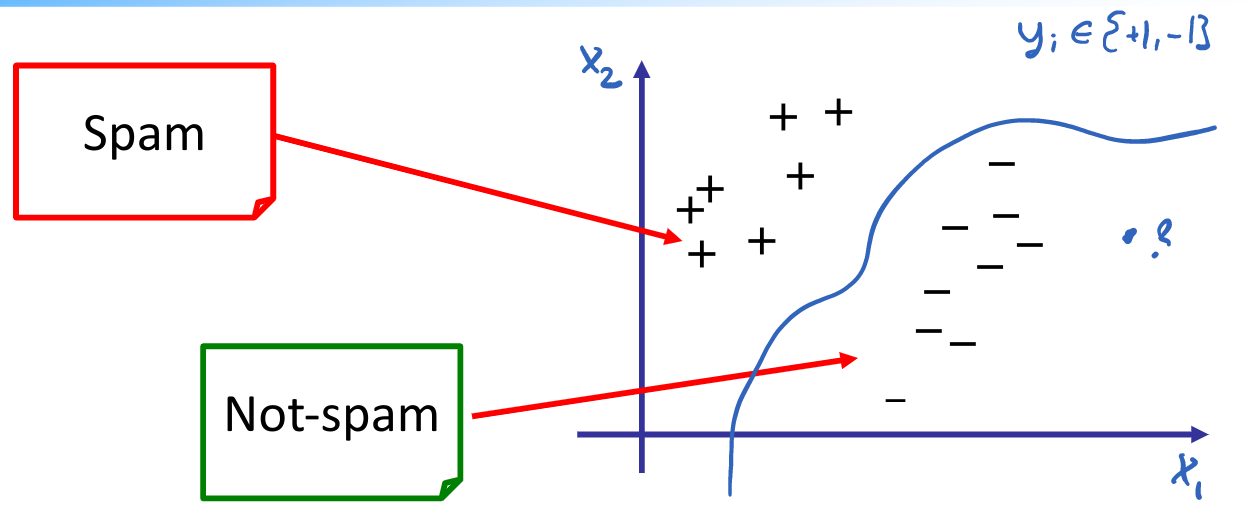
\includegraphics[width=.5\textwidth]{figures/binary_classification.png}
    \caption{Illustration of binary classification}
    \label{binary_classification}
\end{figure}
Given a dataset $D=\left\{(x_1, y_1), \ldots(x_n, y_n)\right\}$, we have:
\begin{equation*}
    y\approx h_{\mathbf{w}}(x)= \text{sign}(w^Tx)
\end{equation*}
Linear classification works well in high-dimensional settings when using the right features; prediction is typically very efficient despite linear classification seeming very restrictive at first.

\subsection{Finding linear separators}

Writing the search for a classifier can be seen as an optimization problem:
we seek the set of weights $\mathbf{w}$ that minimizes the number of mistakes, i.e.:
\begin{align*}
    \hat{\mathbf{w}} &= \arg\min_{\mathbf{w}\in\mathbb{R}}\sum_{i=1}^{n}[y_i\neq \text{sign}(w^Tx_i)]\\
    =\begin{cases}
        1\text{ if } y_i\neq \text{sign}(w^Tx_i)\\
        0\text{ otherwise.}
    \end{cases}
\end{align*}

The goal is then to optimize the following function:
\begin{align*}
    \hat{\mathbf{w}} &= \arg\min_{\mathbf{w}\in\mathbb{R}}\frac{1}{n}\sum_{i=1}^{n}[y_i\neq \text{sign}(w^Tx_i)]\\
    &= \frac{1}{n}\sum_{i=1}^{n}\mathcal{l}(w; x_i,y_i)
\end{align*}
Note that this poses as challenge as it is not convex or even differentiable. Therefore we need to replace this loss by a tractable loss function for the sake of optimization/model fitting. When evaluating a model, we then use the original cost/performance function. The function we can use to optimize in this case is the surrogate loss:
\begin{equation*}
    l_P(\mathbf{w}; y_i, x_i) = \max (0, -y_i\mathbf{w}^Tx_i)
\end{equation*}
which is also referred to as the perceptron loss.

The gradient of the perceptron loss function can be computed as follows:
\begin{align*}
    \hat{R(w)}&=\sum_{i=1}^{n}\max (0, -y_iw^Tx_i)\\
    \nabla\hat{R(w)}&=\sum_{i=1}^{n}\nabla_{\mathbf{w}}\max (0, -y_iw^Tx_i)\\
    &=\begin{cases}
        0\text{ if } y_iw^Tx_i\geq 0 \text{ i.e. correctly classified }
        -y_ix_i\text{ otherwise} 
    \end{cases}
\end{align*}

So we have the following update rule:
\begin{equation*}
    \mathbf{w}_{t+1} \leftarrow \mathbf{w}w_t+\eta_t\sum_{i:(x_i,y_i) {incorrectly classified by} w}^{x_iy_i}
\end{equation*}

\subsection{Stochastic gradient descent}
Computing the gradient requires summing over all data, which is inefficient for large datasets. Additionally, our initial estimates are likely very wrong and we can get a good unbiased gradient estimate by evaluating the gradient on few points. In the worst case, we can evaluate only one randomly chosen point, which is a procedure called stochastic gradient descent. It consists of the following steps:
\begin{enumerate}
    \item Start at an arbitrary $\mathbf{w}_0\in\mathbb{R}^d$
    \item For $t=1,2,\ldots$ do:
    \begin{itemize}
        \item Pick data point $(\mathbf{x}',y')\in D$ from training set uniformly at random (with replacement), and set:
        \begin{equation*}
            \mathbf{w}_{t+1}=\mathbf{w}_t-\eta_t\nabla\mathcal{l}(\mathbf{w}_t;\mathbf{x}',y')
        \end{equation*}
    \end{itemize}
\end{enumerate}
Where $\eta_t$ is called the learning rate. Guaranteed to converge under mild conditions, if:
\begin{equation*}
    \sum_{t}\eta_t=\infty \text{ and }\sum_{t}\eta_t^2<\infty
\end{equation*}
for instance $\eta_t=\frac{1}{t}$ and $\eta_t=\min (c, \frac{c'}{t})$.\\
The perceptron algorithm is just stochastic gradient descent on the perceptron loss function $\mathcal{l}_P$ with learning rate 1.
\begin{theorem}[Perceptron algorithm]
    If the data is linearly separable, the perceptron will obtain a linear separator.
\end{theorem}
The variance of the gradient estimate can be reduced by averaging over the gradients w.r.t. multiple randomly selected points, which are called minibatches. Adaptive learning rates can be additionally applie. There exist various approaches for adaptively tuning the learning rate. Often times, these even use a different learning rate per feature. Examples of adaptive learning rate algorithms include AdaGrad, RMSProp, Adam, ...
\subsection{Hinge loss vs. perceptron loss}
The Hinge loss encourages the margin of the classifier, and is defined as follows:
\begin{equation*}
    \mathcal{l}_H(\mathbf{w}; \mathbf{x}, y)=\max\left\{0,1-y\mathbf{w}^T\mathbf{x}\right\}
\end{equation*}

\section{Support vector machines vs. perceptron}
The optimization objective for the support vector machine is defined as minimizing Hinge loss while also adding another regularization term. There are several lines that need to be considered in the max. margin linear classification, which are summarised in figure \ref{planes_svm}

\begin{figure}
    \centering
    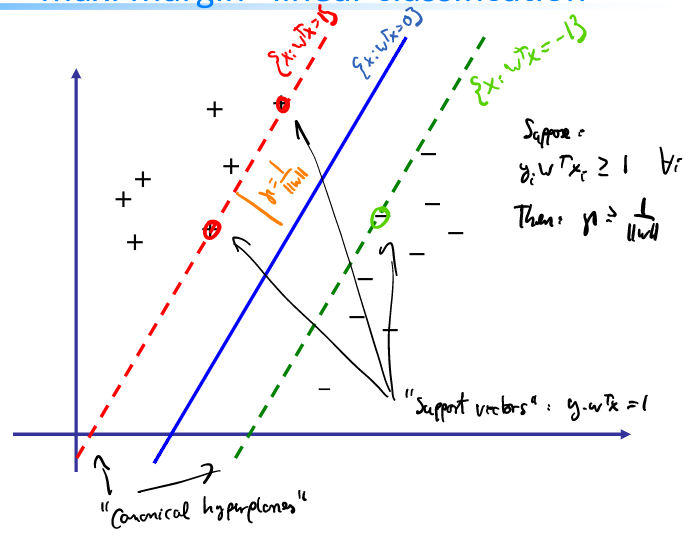
\includegraphics[width=.8\textwidth]{figures/max_margin_decision_boundaries.png}
    \caption{Important elements and their defining equations for support vector machines.}
    \label{planes_svm}
\end{figure}

Support vector machinea re widely used, very effective linear classifiers. They behave almost like a perceptron. The only differences include:
\begin{itemize}
    \item Optimize slightly different, shifted loss (hinge loss)
    \item They regularize the weights
\end{itemize}
It can be optimized using a stochastic gradient descent. A safe choice for the learning rate is:
\begin{equation*}
    \eta_t=\frac{1}{\lambda t}
\end{equation*}
\end{document}